\section{Overview}
\label{overview}

\noindent
In Apache Spark platform, each job consists of multiple execution stages implementing distinct operations of an application program where stages are executed sequentially. To facilitate parallel processing, input data set is partitioned into multiple sets and are distributed over multiple worker nodes. Within each worker node, batches of tasks are launched to process the corresponding partition of the input data. The number of tasks within each node is determined based on the size of the input data and configuration settings of the program. 
\noindent
To illustrate the main idea behind Apache Spark job execution, let us consider the Apache Spark PageRank job running on two worker nodes: A and B, where Node A has 8 CPU cores and Node B has 12 CPU cores as shown in Figure~\ref{flow}. This PageRank job will have 13 stages if the iteration number is set to 10, where stage 1 and stage 2 execute the distinct() operation. In the iteration part from stage 3 to stage 12, the operation reduceByKey() is executed. The final stage performs the saveAsTextFile() operation. As shown in Figure~\ref{flow}, each box in the Figure represents one stage, and each line in the box represents one task. Different colors are used to differentiate tasks running on different worker nodes. If the input data size of this PageRank job is 2.5 GB, the total number of input blocks will be 40 for a default block size of 64 MB. As the number of tasks is same as the input block number, there are 40 lines in each stage. In addition, the number of tasks in each stage is same within one Spark job. Therefore, for this example, in each stage, 40 tasks will be executed. However, different CPU core may complete different number of tasks due to the difference in computing ability and uncertainty during the program execution. 
\noindent
Given the above model of execution, next, we present the developed hierarchical models that can be used to predict job execution time, memory footprint for RDD creation, and I/O overhead as follows. 


\subsection{Model for Estimating Execution Time}

\noindent
As a Spark job is executed in multiple stages where each stage contains multiple tasks, we use the following notation to represent an Apache Spark job:
\begin{IEEEeqnarray}{rCl}
\label{jobperform}
Job &{} ={}& \{Stage_i \mid 0 \leq i \leq M \} \IEEEyessubnumber\\
Stage_i &{} ={}& \{Task_{i,j} \mid 0 \leq j \leq N \} \IEEEyessubnumber%
\end{IEEEeqnarray}
Here $M$ is the number of stages in a job and $N$ is the number of tasks in a stage. 
\begin{figure}[!t]
\centering
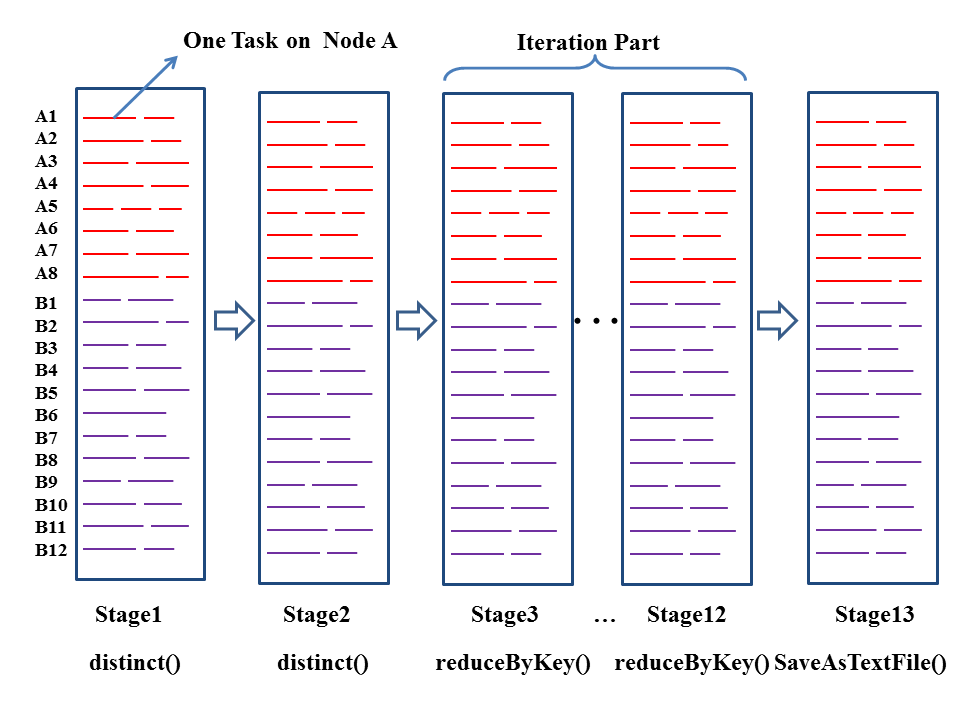
\includegraphics[width=3.0in]{figures/flow.png}
\caption{Prediction Accuracy for WordCount}
\label{flow}
\end{figure}
\noindent
Next, as different stages within a job are executed sequentially, we represent the execution time of a job as the sum of the execution time of each stage plus the job startup time and the job cleanup time as follows:
\begin{IEEEeqnarray}{rCl}
\label{jobtime}
JobTime = Startup + \sum_{s=1}^{M} StageTime_{s} + Cleanup
\end{IEEEeqnarray}
Next, within each stage, as one CPU core executes one task at a time, in a cluster with $H$ worker nodes, the number of tasks $P$ that can run in parallel can be calculated as follows:
\begin{IEEEeqnarray}{rCl}
\label{paralltask}
P=\sum_{i=1}^H CoreNum_{i}
\end{IEEEeqnarray}
Here, $CoreNum_{i}$ is the number of CPU cores of working node $i$ and $H$ is the number of working nodes in the cluster. Hence, within an execution stage, tasks in each stage are executed in batches where each batch consists of $P$ tasks running in parallel. However, due to the differences in computing capabilities among different worker nodes in a heterogeneous cluster and inherent uncertainty in program execution, the execution time of different tasks may vary significantly. Therefore, the time spent in a particular stage can be calculated as the maximum of the sum of all the sequential tasks' time within a stage plus the stage startup time and the stage cleanup time as follows:
\begin{IEEEeqnarray}{rCl}
\label{stagetime}
StageTime&{} ={}& Startup + \max_{c=1}^{P} \sum_{i=1}^{K_c} TaskTime_{c,i} \nonumber \\
&&+Cleanup
\end{IEEEeqnarray}
Here $P$ is the number of total CPU cores, and $K_c$ is the number of sequential tasks executed on CPU core $c$.
Finally, as different tasks in a stage follow the same execution pattern, the execution time of a task can be computed as follows:
\begin{IEEEeqnarray}{rCl}
\label{tasktime}
TaskTime&{} ={}& DeserializationTime + RunTime \nonumber \\
&&+ SerializationTime
\end{IEEEeqnarray}
Here $DeserializationTime$ is the time taken to deserialize the input data, $SerializationTime$ is the time taken to serialize the result, and $RunTime$ is the actual time spent performing operations on data such as data mapping, filtering, calculating, and analyzing. 


\subsection{Memory Consumption}

\noindent
As the Spark platform takes the advantage of in-memory processing to improve the computing efficiency, it is important to allocate sufficient memory needed to create initial RDD to avoid possible slowdown of the execution. Moreover, under certain system configurations, lack of enough memory for initial RDD creation can lead to unexpected program termination. To avoid such adverse events, we develop a simple model to estimate the minimum memory requirement for RDD creation. Specifically, if there are N tasks in the system, we can express the total memory requirement for the job as follows:
\begin{IEEEeqnarray}{rCl}
\label{jobmem}
JobRddMem=\sum_{i=1}^{N} TaskRddMem_{i} 
\end{IEEEeqnarray}





\subsection{Model for Estimating I/O Cost}

\noindent
Finally, within a stage, the transformation operation that generates new RDD based on previous RDD is implemented in $ShuffleMapTask$ and the action operation that output the result data which is implemented in $ResultTask$. The I/O cost during the shuffle phase in these two types of tasks can be classified into two categories, namely, the shuffle read cost and the shuffle write cost. Shuffle write cost is the cost of writing the interim data to local disk buffer, and shuffle read cost refers to the network I/O cost for fetching the interim data from other worker nodes. As shuffle phase is the most I/O intensive phase where frequent data fetching and transmission occurs, in our model, for I/O cost measurement, we specifically focus on data transmission during the shuffle phase that involves data fetching from remote hosts and the interim data writing into the disk. The stage-by-stage I/O cost is calculated as follows:
\begin{IEEEeqnarray}{rCl}
\label{stagewriteio}
StageIOWrite_{i} &{} ={}& \sum_{j=1}^{N} TaskIOWrite_{i,j} \IEEEyessubnumber\\
\label{stagereadio}
StageIORead_{i} &{} ={}& \sum_{j=1}^{N} TaskIORead_{i,j} \IEEEyessubnumber%
\end{IEEEeqnarray}
Here $N$ is the number of tasks in $Stage_i$.



\subsection{ Performance Prediction}
\label{predictsec}

\noindent
Based on the above model, to predict job performance, the presented modeling framework first executes the program on a cluster using limited amount of sample input data and collect performance metrics such as run time, I/O cost, and memory cost during the simulated run. Next, the extracted performance metric from simulated run is used to predict the performance metric for the actual run. 
\noindent
Specifically, to predict the execution time, we first calculate the number of tasks that will be executed in the actual job as follows: $ N = InputSize / BlockSize $, where $InputSize$ is the size of the input data, and $Blocksize$ is the size of one data block in HDFS. 
The tasks within a stage are scheduled to run batch by batch, and the number of tasks in each batch $P$ is computed as shown in equation (\ref{paralltask}). In one batch of tasks, while the tasks may start simultaneously, they may not finish at the same time due to various factors such as data skew problem, and differences in computing capability of different worker nodes. Hence, using simulation data, we calculate the average execution time for a task for a given stage for a worker node $h$ as follows. 
\begin{IEEEeqnarray}{rCl}
\label{taskest}
TaskRunTime_{h,i} &{} ={}& DeserializeTime_{h,i} \nonumber \\
&&+ RunTime_{h,i} \nonumber \\
&&+ SerializationTime_{h,i} \\
\label{avgtask}
AvgTaskTime_h &{} ={}& \frac{1}{n_h}\sum_{i=1}^{n_h} TaskRunTime_{h,i}
\end{IEEEeqnarray}
Here $n_h$ is the number of tasks running in host $h$ in a particular stage of the sample job. 
Moreover, during our experiment, we observed that the average execution time of the first batch is significantly different compared to the subsequent batches within the same stage, which we capture as follows. 
\begin{IEEEeqnarray}{rCl}
\label{ratio}
Ratio_h=\frac{\frac{1}{n_h-P_h} \sum_{i= P_h + 1}^{n_h}TaskTime_{h,i}}{\frac{1}{P_h} \sum_{j=1}^{P_h} TaskTime_{h,j}}
\end{IEEEeqnarray}
Here $n_h$ is the number of tasks running in host $h$, and $P_h$ is the number of tasks in the first batch. Please note that, to trace two batches of tasks to calculate this ratio for every working node, $SampleSize$ needs to be doubled (discussed in Section~\ref{sampling}).
As tasks execute on different hosts in parallel, to predict the execution time for a particular stage during actual execution, stage $Startup$ time and $Cleanup$ time are viewed as constants which are extracted from simulation logs, and stage execution time is estimated as follows: 
\begin{IEEEeqnarray}{rCl}
\label{stageest}
EstStageTime&{} ={}&Startup + \max_{c=1}^{P} \sum_{i=1}^{K_c} AvgTaskTime_{c,i} \nonumber \\
&&+ Cleanup \\
\label{stagetask}
EstTaskTime_{c,i}&{} ={}&\left\{\begin{IEEEeqnarraybox}[\relax][c]{l's}
AvgTaskTime_c,& $i = 1$\\
AvgLaterTaskTime_c,& $i > 1$%
\end{IEEEeqnarraybox}\right.
\end{IEEEeqnarray}
Here $P$ is the number of total CPU cores calculated in equation (\ref{paralltask}), $K_c$ is the number of sequential tasks running in CPU core $c$. $AvgTaskTime_c$ is the average time for tasks in the first batch for CPU core $c$ of the corresponding host, and is calculated in equation (\ref{avgtask}). $AvgLaterTaskTime_c$ is the average time of the following batches of tasks, which could be calculated as $Ratio_h \times AvgTaskTime_h$.
For predicting I/O cost, the average shuffle read and write costs of a typical task is computed and then used to compute the I/O cost for a specific stage j as follows:
\begin{IEEEeqnarray}{lCl}
\label{stageio}
EstStageIOWrite_j \nonumber \\
=\sum_{h=1}^{H} (N_h \times \frac{1}{n_h} \sum_{i=1}^{n_h} (TaskIOWrite_{h,i}))
\end{IEEEeqnarray}
\begin{IEEEeqnarray}{lCl}
\label{stageio}
EstStageIORead_j \nonumber \\
=\sum_{h=1}^{H} (N_h \times \frac{1}{n_h} \sum_{i=1}^{n_h} (TaskIORead_{h,i}))
\end{IEEEeqnarray}
Here $H$ is the number of worker nodes and $N_h$ is the number of total tasks on host h during real execution. $n_h$ is the number of tasks running on host $h$ during simulation at stage j. 
\noindent
Finally, the average memory footprint for each stage is estimated as follows: 
\begin{IEEEeqnarray}{lCl}
\label{stagemem}
EstRddMem = \sum_{h=1}^{H} ( \frac{N_h}{n_h} \sum_{i=1}^{n_h} TaskRddMem_{h,i} )
\end{IEEEeqnarray}


\subsection{Simulation Methodology }
\label{sampling}

\noindent
For simulation, we tried two alternative setup as follows. 
In the first setup, to make sure that all worker nodes in the cluster is used during simulation, we extract sufficient amount of sample input data so that each CPU core gets to process at least one block of input data. Hence, given that one block of HDFS data is configured to be equal to the size $BlockSize$, the minimum value of $SampleSize$ can be calculated as $BlockSize \times P$, where $P$ is the number of tasks that can run in parallel ($P$ is calculated in equation (\ref{paralltask})). 
\noindent
However, as the prediction mechanism needs to extract $2 \times P$ blocks of sample data from the original input to simulate on the whole cluster, for clusters with a large number of worker nodes, total CPU core number $P$ may be very huge, resulting in a big sample job and long simulation time. In order to reduce the simulation time, we tried another alternative where the sample job is executed in a smaller cluster which has fewer number of CPU cores $p$. As a result, only $2 \times p$ blocks of sample data is needed. In our simulation, we ran simulation on a smaller cluster that includes one node of each type (as shown in Figure~\ref{fig:cluster}(b)). Basically, all computing nodes in a cluster can be classified into $D$ groups, where each group has $Num_g$ computing nodes and each computing node in a group has the same computing capability (e.g., CPU speed, RAM). Next, one node is selected from each group, and total $D$ working nodes are chosen to construct this new cluster. In such a setting, the size of sample data is reduced to $D / \sum_{g=1}^{D} Num_g$ times of the original input data, reducing the simulation time significantly. 
Finally, to reduce the impact due to data skew, our sampling technique divides the input data into multiple sections, and extracts data from each section with equal probability.
\begin{figure}[!t]
\centering
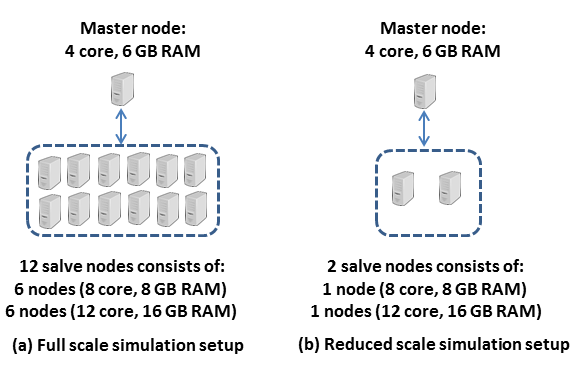
\includegraphics[width=3.0in]{figures/cluster.png}
\caption{Simulation Setup}
\label{fig:cluster}
\end{figure}

